\documentclass{acm_proc_article-sp}
\usepackage{graphicx}
\usepackage{mathtools}
\usepackage{color}
\usepackage[utf8x]{inputenc}
\usepackage{parskip}

\setlength{\parindent}{0pt}
\setlength{\parskip}{\baselineskip}

\begin{document}

\title{Access Control Policy Verification and Repairing in Alloy}

\numberofauthors{1}

\author{
\alignauthor Alexandr Murashkin, Ming Matthew Ma \\
       \affaddr{The David R. Cheriton School of Computer Science}\\
       \affaddr{University of Waterloo}\\
       \affaddr{Waterloo, ON, Canada}\\
       \email{amurashk, m22ma@uwaterloo.ca}
}
\date{6 December 2012}
\maketitle

\begin{abstract}

Important and confidential information can be stored in databases that may be accessible in non-intended way. This heightens the need to carefully control data access: not only preventing the leakage of data but also permitting access to necessary information. Access control requires authorization rules and constraints. To express access control policies, several languages such as XACML are used to specify whether subjects are allowed to access sets of resources or services to perform specific actions. 

We develop a tool based on first-order logic modeling to detect and visualize possible conflicts within sets of access control policies expressed in XACML. We first translate the model into a relational first order logic language called Alloy, and then analyze interactions and conflicts among access control policies using Alloy Analyzer. We then proposes potential repairs to the user through user interface, and automatically apply the fixes selected by the user. We have shown that with our tool can automatically determine inconsistencies in user specified model, prioritize possible fixes and successfully apply the selected repairs to the model. 

\end{abstract}

\category{D.2.4}{Software Engineering}{Software/Program Verification}[formal methods]
\category{H.5.2}{Information Interfaces and Presentation}{User Interfaces}[Graphical user interfaces (GUI)]

\terms{Computer Aided Verification, Access Control Policy, User Interface}

\keywords{access control policy, Alloy, XACML, GUI} % NOT required for Proceedings

\section{Introduction}


Access policy are widely used in systems that require authentication. Data is increasingly available on-line through the Web and other distributed protocols. This heightens the need to carefully control access to data. Access control means not only preventing the leakage of data but also permitting access to necessary information. The key goal is that the right person can access right resource.

\subsection{Motivation}

Due to growing variety of access methods, central databases must now provide data in a
large number of different contexts, each governed by specific access-control policies. Selective access control is an important mechanism in distributed system security. It can be used in order to allow certain users to access only certain information, for certain purposes when he or she plays a certain role. Access control is enforced by mechanisms that need to be programmed by means of policies. An organization may have many such policies, which may have been established at different times, by different people, perhaps without a clear view of all the consequences. Inconsistencies can then exist in such sets of policies. 

While policy mechanisms may be able to solve inconsistencies at a higher level, users and administrators still need to be aware of them, because they may lead to unintended system behavior. For example, a policy may be added to prevent a certain access, however in fact the access is still allowed because of another policy of higher priority, or the new policy may prevent access of someone who should remain authorized. We will show in this paper that such inconsistencies can be detected and fixed by using our tools.

\subsection{Background}

\subsubsection{XACML access control policies}

XACML is OASIS standard and stands for eXtensible Access Control Markup Language \cite{oasis:xacml}. It defines structure, interaction and conventions related to policy sets, policies, rules and request within an access control system. XACML generally centers around attributes: attributes describe subjects, actions, and resources. Subject can be described by the $Role$ attribute, resource by its $ResourceName$, and action by its $ActionName$. Usually XACML access control policies are stored in XML files. The names of attributes, such as role are called $AttributeId$, while the values bound
to them are called attribute values  (such as $Professor$). The shortened fragment of an XACML policy designating $Professor$ as a role is shown below:\\

\begin{verbatim}
<Subject>
  <SubjectMatch MatchId="...:string-equal">
    <AttributeValue
      DataType="...#string">Professor</AttributeValue>
    <SubjectAttributeDesignator
      AttributeId="role"
      DataType="...#string"/>
  </SubjectMatch>
</Subject>
\end{verbatim}

If we consider more coarse-grain structures, access control policies are structured into rules, policies and policy sets. Several rules are grouped into policies and policies are grouped into policy sets. Rules, policies and policy sets define a target which indicates their domain of applicability. A target specifies a set of attributes and their values that should match those given by a request. A rule in XACML specifies which decision to take and it is a function of the attributes. The XACML takes in a request, names and values of a set of attributes, and makes an access-control decision on it based on the specified rules. A decision can be $permit$, $deny$, or $not-applicable$ which indicates that the request is not handled. 

XML-files are complex, so for our example we can use tabular form of defining policy sets (it is not commonly used, but it is more compact and straight-forward in out case), see Fig.\ref{fig:policyset}.

\begin{figure}[h]
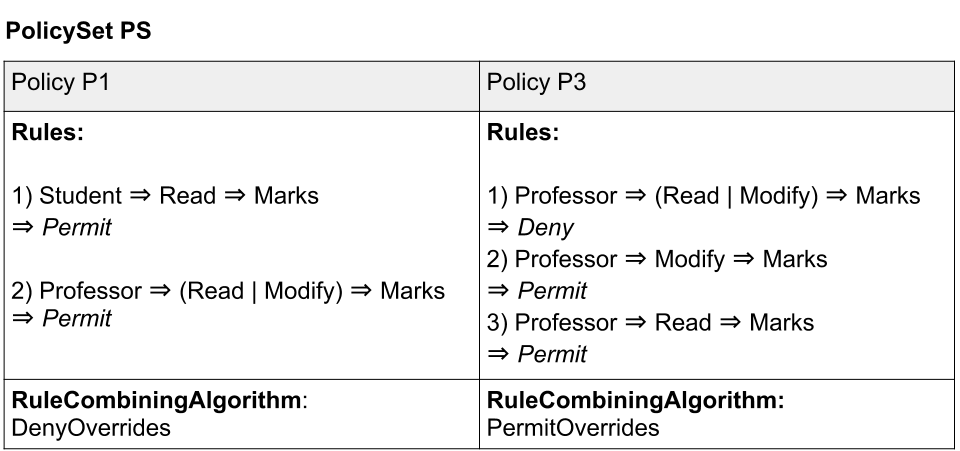
\includegraphics[width=0.5\textwidth]{policyset.png}
\caption{Policy Set PS contains two policies: P1 and P3, each has a set of rules and rule combining algorithm}    
  \label{fig:policyset}
\end{figure}

So, in our example a policy set $PS$ contains two policies: $P1$ and $P3$, the first rule of $P1$ is $Student \to Read \to Marks \to Permit $ is applied when the subject has the role $Student$, the resource is the $Marks$ file and the action is $Read$, and this access is granted ($Permit$). In policy $P3$, the first rule denies both reading and modifying marks for professor. The policy has $DenyOverrides$ rule combining algorithm which says that this rule is dominant over others in case that more than one rule is applicable for some relevant request. The policy response is equal to the one rule which is applicable or by the dominant rule if multiple rules are applicable. The same is true for policy set response, but it has $OnlyOneApplicable$ policy combining algorithm as well, which says that the policy set response in indeterministic if more than one policy is applicable in the context of a given request.

\textbf{\emph{Alloy}}\\
Alloy \cite{jackson:alloy} is a modeling language based on relational first order logic. An Alloy model is a collection of constraints that describes a set of structure. Alloy's tool, the Alloy Analyzer, is a solver that takes the constraints of a model and finds variables that satisfy them. It can be used both to explore the model by generating sample structures, and to check properties of the model by generating counterexamples. 

To model structures, Alloy uses the concepts of signature and relation. A signature is a type in Alloy. It can be considered equivalent to a class in the object oriented paradigm since a signature can be instantiated. For example, we can define a policy P1 as follows \cite{acp:alloy}:
 
 \begin{verbatim}
abstract sig Policy {
  policyTarget : one Target,
  rules : set Rule,
  combiningAlgo : one RuleCombiningAlgo
} 
\end{verbatim}

A relation is a structure that relates signatures and their instances. Functions are special binary relations; they map each instance from the left signature to only one instance from the right signature (the function effect maps each rule to only one effect). Constraints are represented in Alloy by facts. A fact is a logical formula that always holds. Alloy uses first order logic in an ASCII format. We can also specify predicates that could be evaluated to return true or false and functions that could return signature instances. Alloy is able to automatically instantiate and evaluate predicates.

\section{Problem Statement}

Although XACML has already achieved a considerable degree of industrial acceptance, by itself, it is impossible to determine inconsistencies and apply the fixes to repair the access control model. Inconsistencies exist as an organization may have many such policies, which may have been established at different times, by different people, perhaps without a clear view of all the consequences. 

Determining inconsistencies require verifications and finding counterexamples. This process is time-consuming depending on the choice of verification and modeling language. Once inconsistencies are found, the user has to apply fixes but there is no guarantee that the fixes can indeed repair the model without introducing new inconsistencies. Thus, the entire model construction process, model verification process, finding inconsistencies and repairing process can be overwhelming.

In this paper, we propose a tool that we developed that can automatically determine the inconsistencies, recommend the repair to the users and apply fixes to the access control model.

\subsection{Related work}

Regarding access control policy verification, there are several various related approaches.
\cite{Hughes:2008:AVA:1459278.1459282} proposed encoding XACML access control policies  ordering relations and then translation of them into SAT solver for verification. This paper defined some Alloy notation as well.  The papers \cite{acp:automated} and \cite{acp:alloy} defined XACML access control policies notation in Alloy and deal with verification problem. The latter approach - \cite{acp:alloy} - is used in our paper, it introduces the usage of predicates for access control policy model verification and validation. We found the way the models are defined in this paper straight-forward, so we used this approach and extended it. Other than that, \cite{4258517} describes inconsistency checking in role-based access control policies (RBAC). \cite{Fisler:2005:VCA:1062455.1062502} proposes Margrave - a tool for access control policies (XACML and other formats) verification and change-impact analysis. \cite {acp:descriptionlogics} used description logics to formalize and verify access control policies. The authors also specified semi-automated access control policy repair as their future work.

None of the paper above solves the problem of access control policy repairing. It does not seem to be published prior related work in this topic. Rather than that, \cite{Zhang:2004:SVA:1029133.1029141} offers access control policies verification in the language called RW and then synthesize verified specifications in XACML. \cite{Bravo:2007:RIX:1783534.1783545} considers another type of access control policies - XML write access control policies - offers repairs in case of that some actions can be simulated by multiple another actions. Regarding repair in general and different domains, \cite{Reder:2012:CRT:2351676.2351707} proposes repair trees for inconsistency solving in design models. We use similar trees in our repairing approaches. There are works on model repairing in temporal logic, but we do not consider the notion of time in our work. Semi-automated repairing of XACML access control policies is the most important contribution of this paper. 

\subsection{Paper structure}
The Implementation section gives brief overview of our we will introduce verification and model repairing approaches we took for the implementation of our tool. We will present the main components of our tool and the implementation at different stage. Evaluation section contains our toy experiment results. In future work section, we discuss our tool limitations and bring up possible future improvements. Conclusion section summarizes completed work and achieved results.

\section{Implementation}

In this section, we present the verification and repair approaches, architecture and data flow of the tool in details.

\subsection{Verification approach}

The verification procedure is based on the one in the technical report \cite{acp:alloy}. We use the same idea in our paper.
The first step is to define the Alloy input file.

1. First, a meta-model (or abstract model) is defined at the beginning of the file. This meta-model is domain-specific. It consists of signatures ($Policy$, $PolicySet$, $Rule$, $Effect$, $RuleCombiningAlgorithm$, etc.) and relations ($rules$ relation links a policy and rules it contains).

2. Next, a concrete model is defined. It consists of signatures ($Policy1$, $Policy2$, $Rule1$, $Rule2$) and facts ($Policy1$ contains $Rule1$ and $Rule2$) regarding the relations specified in meta-model. Concrete model can vary within the given domain, so one meta-model can be used for many concrete models within the domain.

3. And finally, a property predicate is defined. This predicate is domain-specific as well, and each predicate represents the negation of the property we need to verify. In this paper, we focused on an abstract property. It is stated as follows: within a policy set that has $OnlyOneApplicable$ policy combining algorithm, there is no two policies that for a given request return different decisions. The full body of the predicate is given in the Appendix, and its signature looks as follows:

\begin{verbatim}
pred InconsistentPolicySet [ps : PolicySet, 
    req : Request,  p1: Policy, p2: Policy, 
    r1: Rule, r2: Rule]
\end{verbatim}

The predicate is supposed to find a policy set $ps$ that has $OnlyOneApplicable$ policy combining algorithm and contains policies $p1$ and $p2$, such that policy $p1$ contains rule $r1$, policy $p2$ contains rule $r2$. At the same time, $r1$ defines the response of policy $p1$: the rule $ r1$ is either the only applicable rule in context of the given request $req$, or dominates all other rules of the policy $p1$ after apllying the rule combining algorithm. And similarly, $r2$ defines the response of policy $p2$.

And the second step is to send the Alloy file to Alloy Analyzer and execute the property predicate. We will denote the part of Alloy file without predicate as a model (so, the model consists of two parts: abstract model and concrete model). If the model is consistent, then the predicate is inconsistent with respect to the model, and Alloy Analyzer cannot generate an instance (example). If the predicate is consistent, it means that the model is inconsistent with respect to the property (the property is not satisfied in the model), and a counterexample is returned.

This verification approach gives certain advantages. We can localize the inconsistency, since Alloy Analyzer will show the values of all the arguments of the predicate in the generated instance, including the request $req$, even if there is no definition of request. It is not the case if we make the predicate denote the property itself, not its negation: in this case, if the property is not satisfied, then $UNSAT$ cores can be shown, but it takes computation time to minimize them, and they still might not be minimal. So, for error localization the taken approach is better.

\subsection{Repair}

Once there is an inconsistent policy set, the verification procedure will return the policy set $ps$, policies $p1$, $p2$ and the corresponding rules $r1$ and $r2$. Our repair procedure is applied to policies or rules, and this will affect the consistency of the policy set $ps$. Since our verification procedure returns two rules of two policies, actually we can try to apply the same set of repairs to each of them by simmetry. Therefore, we can consider the following simple repair ways in the context of the returned policy set $ps$, and one policy $p1$ and rule $r1$ within it.

\begin{enumerate}
\item Switch the effect of the rule $r1$. If it was $Permit$, it is changed to $Deny$, and conversely.
\item Switch the policy combining algorithm of the policy $p1$. If it was $PermitOverrides$, it becomes $DenyOverrides$, and conversely.
\item Remove the rule $p1$ from the policy $p1$.
\item Remove the policy $p1$ from the policy set $ps$.
\item Switch the policy combining algorithm of the policy set $ps$ from $OnlyOneApplicable$ to either $DenyOverrides$ or $PermitOverrides$.
\end{enumerate}

The ways 1 and 2 seems to be the best. Just switching the values is definitely less radical. Ways 3 and 4 are dangerous: first, they might affect other requests; next, they can bring us to the empty model which satisfies everything. Way 5 is quite global to apply it, and again, it will hide the conflicts at all, and this can cause more problems in the future. There can be other ways, though: changing the subject, action and resource, but this is risky and can increase the number of states. 

So, for this project, we end up with the first two repair ways and we can apply them to both $p1$ and $p2$, so actually we have 4 repair ways:

\begin{enumerate}
\item Switch the effect of the rule $r1$.
\item Switch the policy combining algorithm of the policy $p1$.
\item Switch the effect of the rule $r2$.
\item Switch the policy combining algorithm of the policy $p2$.
\end{enumerate}

However, the application of one repair way might not be enough, in case that the core of inconsistency is not represented by two rules only. First, there might be redundant rules. For example, if the rule $Student \to Read|Modify \to Marks \to Permit$ is present, then the rule $Student \to Read \to Marks \to Permit$ is redundant, and changing the rule effect of the latter will cause the application of the former rule and this will not solve the problem in one step. This case is handled during the optimization during the conversion of the source file to Alloy file. Next, there are cases that a policy set is faulty for more than one request (not only for the request $Professor \to Read \to Marks$, but with the request  $Professor \to  Modify \to Marks$, for instance), and it definitely needs more than one repair procedure in our approach. This is why we propose the displaying of the approximate numbers of next fixes.

The approximate number of next fixes is calculated as follows. After repairs have been proposed, the system tries to apply each of them gaining partially repaired models. Then, it runs the verification again for each of the partially repaired models. If some partially repaired model is consistent, it means that this model is fully repaired. So in this case, the approximate number of next fixes is zero. If some partially model is still inconsistent, then the system tries to apply fixes to the partially repaired model again, and adds 1 to the number of next fixes. This process can run infinitely and cause state explosion problem, so we limit the depth to certain amount (in our case we specified 2).

If the number of next fixes for each fix is greater than zero, then user needs to apply fixes multiple times. The user will go down the repair tree until he will get the fully repaired model.

In this approach, more than one path can produce the repaired model. It does not matter whether this is a minimal one or not: if the user chooses the path with minimal number of next fixes, then eventually he will get the repaired model with minimal number of changes.

However, there is a problem with this approach - cycles. For example, switching rule combining algorithm may not be helpful. So the system will propose to switch rule combining algorithm and then, at the next step, switch it back. However, our approach helps to solve this problem: if cycles are present, then the way that leads to cycles will be annotated with bigger number of next fixes automatically, so it is less likely that the user will want to choose this way.

\subsection{Tool implementation overview}
The function of our tool is to automatically determined inconsistencies within access control policy defined by XACML, and recommend the potential repair to the user, and finally apply the user chosen fixes automatically. Throughout this process, user only have to review the recommended fixes, and choose the fix by clicking a button in user interface, and then the model should be fixed automatically by our tool. 

To increase the usability of our tool, we have an external module, a converter that can automatically generate Alloy model based on a table template (or xml, csv file template) so that the user does not need to have complete literacy in Alloy modeling language. As the content of the such a template, the user is asked to specify the rule, subject, action, resource and effect in predefined format. Our converter will than generate the Alloy model and its predicate to verify inconsistencies, which is a safetyness property. Once Alloy model is generated, we input the model into our inconsistency detection and repair tool. 

\subsection{Architecture and data flow}

Our tool consists of three major parts: the User Interface (UI), PropertyVerifier\&Fixer and Alloy Analyzer. The architecture is shown in the figure below (Fig.\ref{fig:Architecture}).\\

\begin{figure}[h]
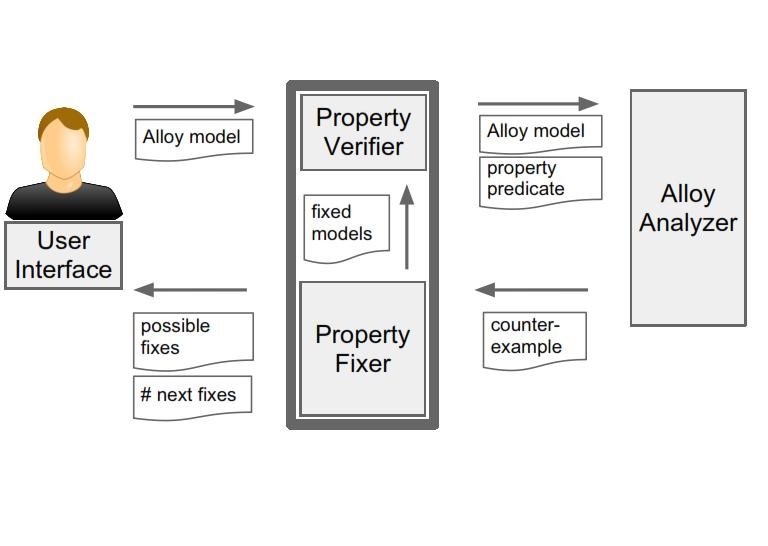
\includegraphics[width=0.5\textwidth]{DataFlow.JPG}
\caption{Tool Architecture and Data Flow}    
  \label{fig:Architecture}
\end{figure}

At the beginning, the UI first takes in the Alloy model created, and sends it to PropertyVerifier\&Fixer. Next, the PropertyVerifier part starts Alloy analyzer to process Alloy model and its property predicate. It should be noted that we write our predicate in a way that it checks for if two policies return inconsistent results. PropertyFixer then takes in the results from Alloy Analyzer and extracts relevant information, such as inconsistent rules, subject, action, resource and effect, and process those information to propose the potential fixes. The fix recommendation from PropertyFixer is passed to the UI, and the user is shown with a list of fixes. Once the user chooses one particular fix, our tool will automatically update the original Alloy model. This updated model is then passed to PropertyVerifier to check if there are any inconsistencies. This process is repeated until the model is verified to be consistent.

In order to realize the above mentioned architecture, we have created several Java modules which are summarized below.

\subsubsection{InteractiveRepairer}
This is the core of our tool, it contains:
\begin{itemize}
\item Main engine
\item PropertyVerifier
\item PropertyFixer
\end{itemize}
The Main engine controls the communication between the user interface and our Fixer and Verifier; it process input from UI and outputs the results to UI for user inspection. PropertyVerifier calls Alloy Analyzer through our API and obtains XML representation of the generated instance that contains information about the policies, rules, request and effects. PropertyVerifier then follows XPATH standard to extract and store that information from XML for later processing. Once the XML nodes are extracted with relevant information from Alloy Analyzer, PropertyFixer takes in those information and proposes potential fixes. Once the user selects the preferred fix, this decision is communicated to PropertyFixer again through Main engine, and PropertyFixer will automatically apply the fixes to the original Alloy model.

Note that PropertyFixer and PropertyVerifier function as a pair, and one pair is required for each property to be verified; in our study, we limit the property verification to the safety property but this is extensible by creating another pair of PropertyFixer and Verifier.

\subsubsection{AlloyRunner}
AlloyRunner is an API that facilitate the communication between our tool with Alloy analyzer. Mainly, it initializes the Alloy Analyzer, sends model to Alloy analyzer, and get XML instances from Alloy Analyzer. Alloy Analyzer serves as verification engine for our input model and will return instances or counter example which we use in later processing.

\subsubsection{Presentation Layer}
Presentation uses dynamic web application technologies such as Javascript and Node.js to allow interactive model repair. Node.js executes interactive repair with user inputs and calls back to the Main engine in InteractiveRepairer to apply the repair. For instance, the Propose button triggers Main engine to start PropertyVerifier to execute the model verification, and the Resolve links will cause the PropertyFixer to apply the repair on the original Alloy model. The return values are associated with each function call-back of the button, and represents error location and proposed fixes for Propose command and new model for Resolve command. All proposed fixes are shown and annotated by the approximated number of next fixes.

\section{Evaluation Result}

\subsection{Form and purpose}

ToBeAdded

\subsection{Results}
ToBeAdded

\section{Future work}

Although our tool demonstrate potential value in automated access control model repair, while significantly reducing user's manual work, we see future improvements in our tool. We noticed the following limitations in our tool:

\begin{enumerate}
\item Verification is bounded
\item Can verify one property in a time until first counterexample is found
\item Subset of XACML is covered
\item Repair procedure depends on the property and requires pre-defined prospective repair ways
\end{enumerate}

The first two points are pretty clear. Since we use Alloy as it is for bounded model checking, we can guarantee that the tool will give correct results within the given scope. Although we significantly dependent on Alloy, we mainly interfaced the communication with Alloy API, so in the future, we need to communicate with Alloy back-end to prevent this problem.

Although we strive to make our tool scalable, the automated Alloy model generation from a user specified table brings limitations in the structure of the model we generate. Although this access control model works well for our present study, it only represents a subset of XACML. In the future, we would like to explore different ways to increase the flexibility of our model. One potential way is to incorporate sketching techniques and having multiple rule tables so that the user can choose the structure of the model our tool generates.

State explosion is not addressed in a smart way due to time constraints. By now, we use repair trees and limit the depth of the potential solution to two. This might still bring problems if the model is large and the number of fixes is big. We would like to study more on ways to deal better with this common problem in verification and repair.

One important future improvements is on the repair recommendation. Currently, we only proposes repairs based on rule effect and combining algorithm. We derived these approach from observation and testing. We will explore other factors such as relation, and derivation in the future to enhance our repair framework.

\section{Conclusion}

\subsection{Summary}
In this report, we presented our tool which can automatically determine inconsistencies in XACML access control policy, recommend the fixes to the user and automatically apply the repair on the model. We allow user interaction by an user interface where we display our fixed results, Alloy model and also obtain user input.

We have created the input converter so that user can just specify the policies in our provided format in CSV, table form, and we will automatically generate Alloy model for the access control policy, reducing the manual work and user knowledge on Alloy as a modeling and verification tool. Our tool takes in the Alloy model and run Alloy analyzer in the back-end, and retrieve the information on generated inconsistency instances to propose potential fixes. Among the fixes, we also show the total number of fixes required for the selected fix. From evaluation result, it is proved that our tool can help the user to repair inconsistent access control policy model effectively, requiring only user input for fix selection as a manual part. 

\subsection{Implications}

From our project, we conclude that ``automated'' model repair is possible for access control policy defined by XACML structure. We make implications on the fact that user input is still necessary to reduce the redundant computation and steps taken to fix the model. By allowing user to select from list of recommended fixes, and use the user input as new argument in our automated repair tool, we are able to efficiently repair the model without looping.

One other implication we make is that our tool should be easily extensible so that the model repair is not limited to access control policy. We see our InteractiveFixer module as a ``head'' which we can change according to the targeted model that needs to be verified. 


\bibliography{sigproc-sp}{}
\bibliographystyle{plain}

\appendix
\section{Verification property predicate, Alloy syntax} \label{A}

\begin{verbatim}

pred InconsistentPolicySet [ps : PolicySet, 
    req : Request,  p1: Policy, p2: Policy, 
    r1: Rule, r2: Rule]{

  ps.combiningAlgo = P_OnlyOneApplicable 
  p1 in ps.policies
  p2 in ps.policies
  p1 != p2
  r1 in p1.rules
  r2 in p2.rules
  policyResponse[p1, req] = Permit
  (
    p1.combiningAlgo = DenyOverrides and
    (no r1':Rule | r1' in p1.rules 
      and ruleResponse[r1', req] = Deny)
    and ruleResponse[r1, req] = Permit
  )
  or
  (
    p1.combiningAlgo = PermitOverrides
    and ruleResponse[r1, req] = Permit
  )
  policyResponse[p2, req] = Deny
  (
    p2.combiningAlgo = PermitOverrides and
    (no r2':Rule | r2' in p2.rules 
      and ruleResponse[r2', req] = Permit)
    and ruleResponse[r2, req] = Deny
  )
  or
  (
    p2.combiningAlgo = DenyOverrides
    and ruleResponse[r2, req] = Deny
  )

}

\end{verbatim}



\balancecolumns
\end{document}
